\documentclass[a4paper,12pt]{article}
\usepackage[utf8]{inputenc}
\usepackage[cm,empty]{fullpage}
\usepackage[T2A]{fontenc}
\usepackage[english, russian]{babel}
\usepackage{amssymb,amsmath,amsxtra,amsthm}
\usepackage{proof}
\usepackage[pdftex]{graphicx}
\usepackage{wrapfig}
\usepackage{braket}
\usepackage{xcolor}
\usepackage{enumitem}

\usepackage[left=2cm,right=2cm,
    top=1cm,bottom=1cm,bindingoffset=0cm]{geometry}

\renewcommand{\leq}{\leqslant}
\renewcommand{\geq}{\geqslant}


\newcommand{\iiff}{\Longleftrightarrow}
\renewcommand{\iff}{\Leftrightarrow}
\newcommand{\nothing}{\varnothing}

\newtheorem*{rem}{Замечание}

\newcommand{\NN}{\mathbb{N}}
\newcommand{\ZZ}{\mathbb{Z}}
\newcommand{\Q}{\mathbb{Q}}
\newcommand{\A}{\mathbb{A}}
\newcommand{\R}{\mathbb{R}}
\renewcommand{\C}{\mathbb{C}}

\renewcommand{\phi}{\varphi}
\newcommand{\eps}{\varepsilon}

\makeatletter
\newcommand*{\rom}[1]{\expandafter\@slowromancap\romannumeral #1@}
\makeatother

\newcounter{z}


\newcommand{\zs}{\refstepcounter{z}\vskip 10pt\par\noindent
\fbox{\textbf{12.\arabic{z}}} }

\newcommand{\z}{\refstepcounter{z}\vskip 20pt\noindent
\fbox{\textbf{\arabic{z}}} }

\renewcommand{\date}{{\bf 2 июля 2021}} 

\newcommand{\dif}
{
------------------------------------------------------------------------------------------------------------------------------------------------------
}

\newcommand{\HSEhat}{
\vspace*{-0pt}
\noindent
\setcounter{z}{0}


{\bf \phantom{\date}  \large \hfill Прикладная статистика: \hfill \normalsize \date}

\vspace{5 pt}
{\bf \large \hfill  задание 2\hfill }

\vspace{15 pt}
\centerline{ \large  Домашнее задание.}
\centerline{ \large  Кирилл Сетдеков}



\vspace*{10pt}
\setcounter{z}{0}

}

\begin{document}
\HSEhat


\begin{enumerate}

\subsection*{Задачи:}

\item С помощью неравенства Чебышёва покажите,с какой вероятностью величина лежит $[\mu - 2 \sigma, \mu + 2 \sigma]$ и  $[\mu -3 \sigma, \mu +3 \sigma]$.
Сравните полученные вероятности с соответствующими вероятностями для стандартного нормального распределения N (0, 1). Какой вывод можно сделать?

\textbf{Решение:}\\
Формулировка неравенства Чебышева:
$$P(|X-\mu| \geq a) \leq \frac{\sigma ^2 }{a^2}$$
Нас интересует обратная вероятность:
$$P(|X-\mu| < a) > 1- \frac{\sigma ^2 }{a^2}$$

Подставим значения для 2 сигм, заменив $a = 2 \sigma$:
$$P(|X-\mu| < 2 \sigma) > 1 - \frac{\sigma ^2 }{4 \sigma^2} = 1-\frac{1}{4} = \frac{3}{4}=0.75$$

Из нормального распределения: $P(|X-\mu| < 2 \sigma) = \Phi(2) - \Phi(-2) = 0.9545$

Аналогично для 3 сигм, заменив $a = 3 \sigma$:
$$P(|X-\mu| < 3 \sigma) > 1 - \frac{\sigma ^2 }{9 \sigma^2} = 1-\frac{1}{9} = \frac{8}{9} \approx 0.889$$
Из нормального распределения: $P(|X-\mu| < 3 \sigma) = \Phi(3) - \Phi(-3) = 0.9973$

\textbf{Ответ: с помощью неравенства Чебышёва оценки для этого интервала имеют меньшую вероятность, чем вероятности, используя функцию распределения стандартного нормального распределения. $\Rightarrow$ если мы знаем форму распределения, лучше считать через его квантили так как оценка будет точнее, а неравенства Чебышёва использовать в случаях, когда мы совсем ничего не знаем про распределение} 

\item Пусть есть реализация выборки $x_1, ... , x_n$ из $Unif([0,\theta])$ с неизвестным $\theta$.

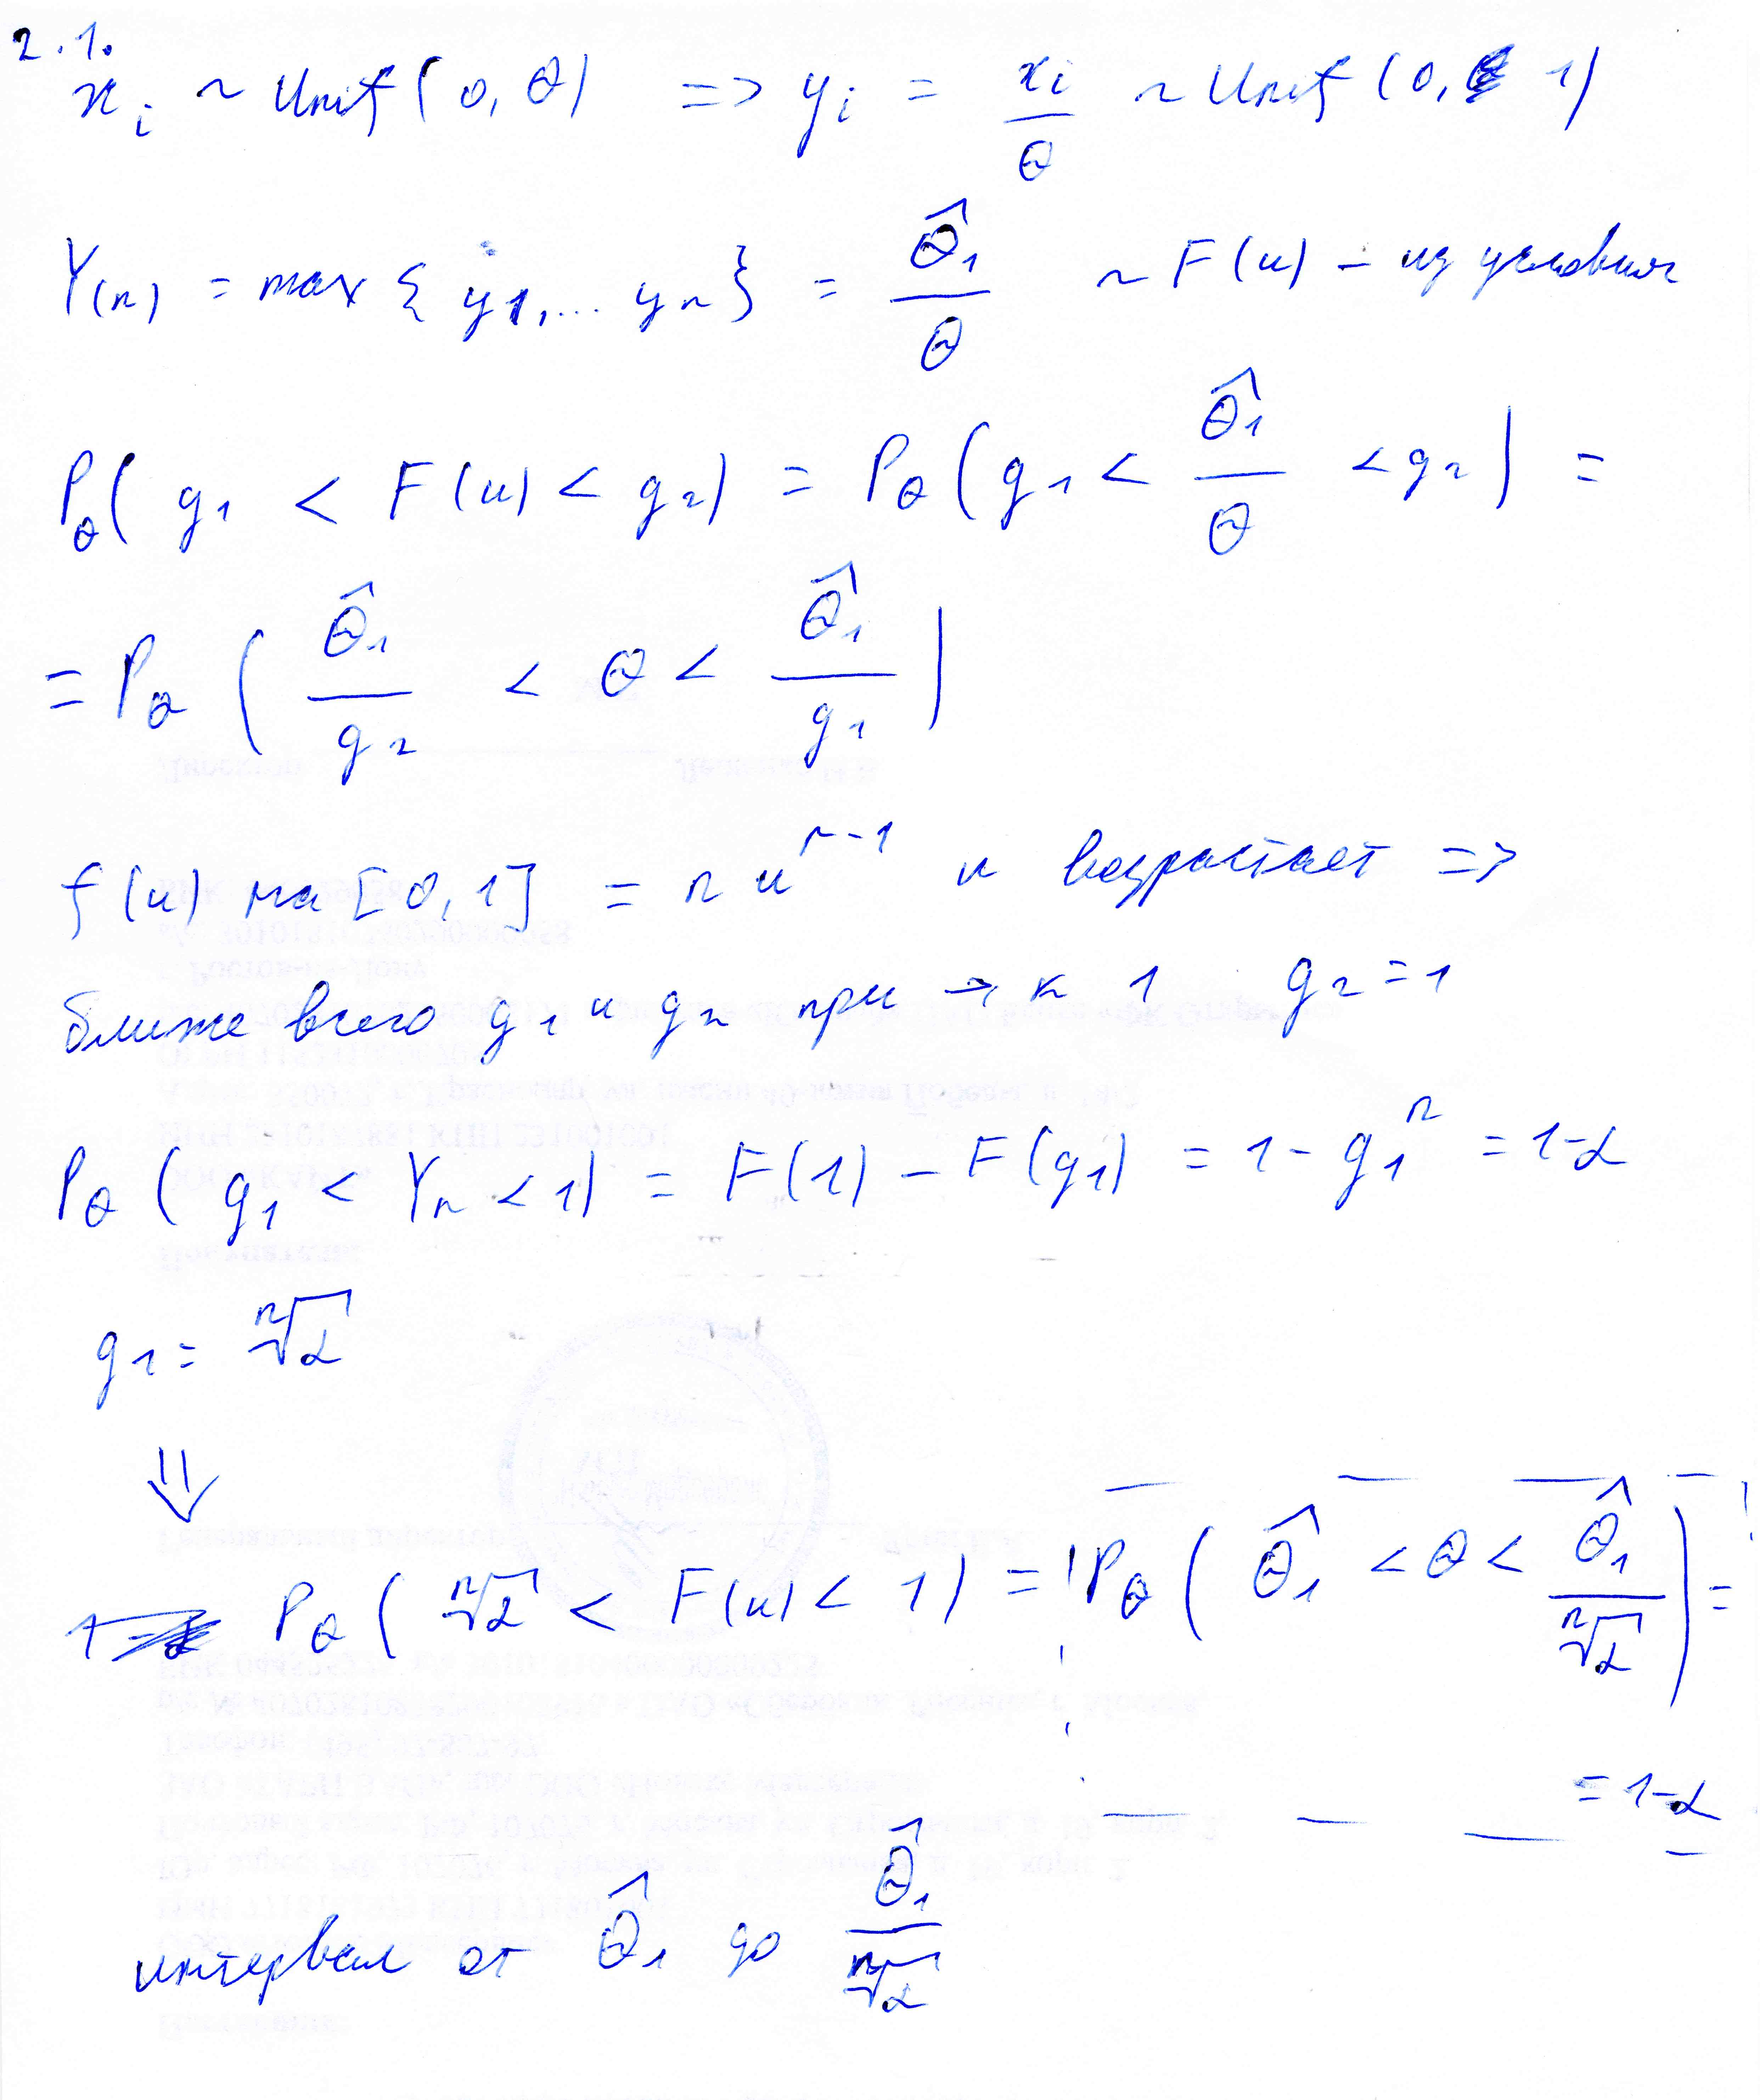
\includegraphics[width=\textwidth]{img/21.jpg}
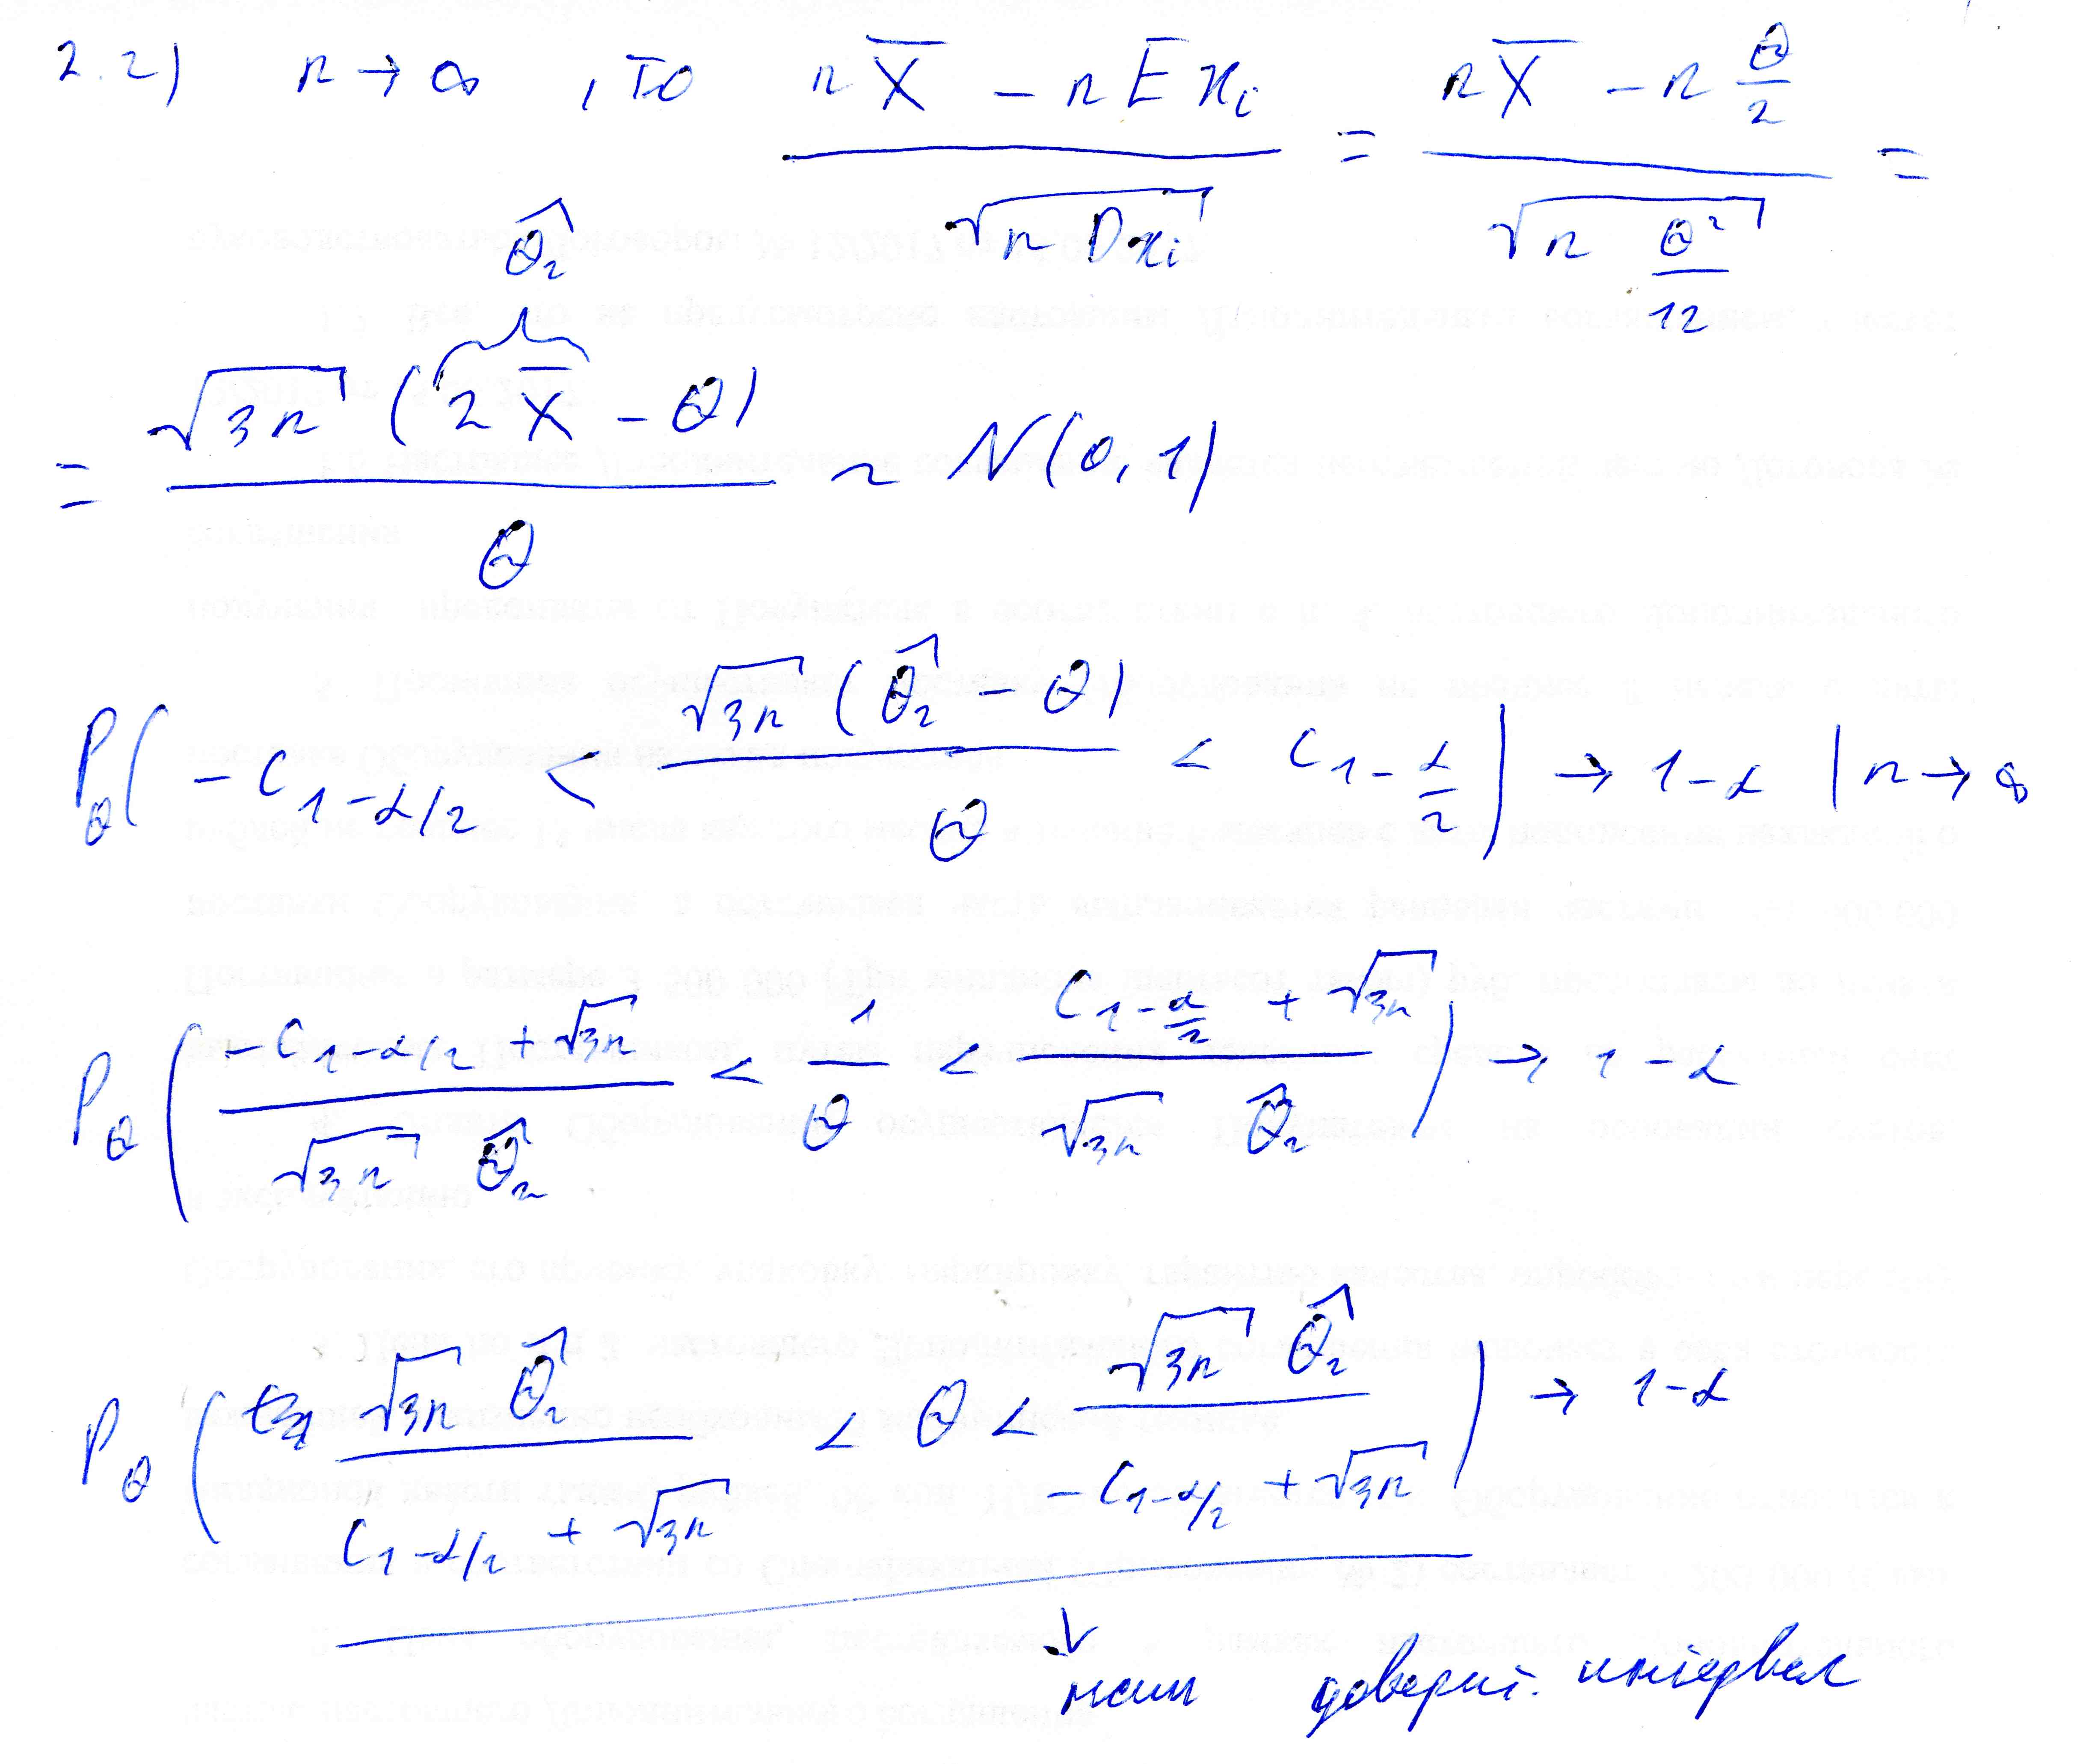
\includegraphics[width=\textwidth]{img/22.jpg}

\item Про выборки

\item Про оценки для среднего в нормальном распределении, реализация на питоне.

Я решил и описал это задание в приложенном ноутбуке.




\end{enumerate}
\end{document}